% =====================================================================
%  BÀI BÁO KHOA HỌC — Payment Intelligence Ecosystem
%  Biên dịch: xelatex bai-bao-khoa-hoc.tex (2 lần để có tham chiếu chéo).
%  Hình dùng chung thư mục figures/ với bao-cao-thuc-tap.tex.
% =====================================================================
\documentclass[11pt,a4paper]{article}

\usepackage{fontspec}
\setmainfont{TeX Gyre Termes}
\setsansfont{TeX Gyre Heros}
\setmonofont{DejaVu Sans Mono}[Scale=0.82]
\usepackage[vietnamese]{babel}
\usepackage{amsmath,amssymb,amsthm}
\usepackage[a4paper,margin=2.5cm]{geometry}
\usepackage{setspace}\setstretch{1.12}
\setlength{\emergencystretch}{3em}
\usepackage{graphicx}
\usepackage{booktabs,tabularx,array}
\usepackage{enumitem}\setlist{nosep,leftmargin=1.5em,topsep=0.3em}
\usepackage{caption}\captionsetup{font=small,labelfont=bf,skip=4pt}
\captionsetup[table]{position=top}
\usepackage{float}
\usepackage[hidelinks]{hyperref}
\usepackage{xurl}
\usepackage{titlesec}
\titleformat{\section}{\large\bfseries}{\thesection.}{0.5em}{}
\titleformat{\subsection}{\normalsize\bfseries}{\thesubsection.}{0.5em}{}
\titleformat{\paragraph}[runin]{\normalsize\itshape}{}{}{}[.]
\titlespacing*{\paragraph}{0pt}{0.4em}{0.5em}

\theoremstyle{definition}
\newtheorem{definition}{Định nghĩa}
\theoremstyle{remark}
\newtheorem{remark}{Ghi chú}

\newcommand{\code}[1]{\texttt{#1}}
\numberwithin{equation}{section}
\renewcommand{\arraystretch}{1.2}

\title{\textbf{Đánh giá trung thực cho phát hiện gian lận\\ và giám sát độ ổn định thanh toán:\\ một nền tảng dữ liệu tái lập được}}
\author{Đỗ Trung Tuyến\\[2pt]
\small Báo cáo thực tập\\
\small \href{mailto:trungdo2002.hvt@gmail.com}{\texttt{trungdo2002.hvt@gmail.com}}\\
\small \url{https://github.com/TrungTuyenDo02/Payment_Intelligence_Ecosystem}}
\date{Tháng 11 năm 2026}

\begin{document}
\maketitle

\begin{abstract}
\noindent Bài báo trình bày một nền tảng dữ liệu nhỏ cho mảng thanh toán, chạy hoàn toàn trên máy cá nhân, gồm hai ứng dụng: (i) giám sát độ ổn định của hệ thống thanh toán trên dữ liệu sự kiện giả lập có cài sẵn sự cố, và (ii) chấm điểm rủi ro gian lận trên dataset công khai IEEE-CIS (590.540 giao dịch, khoảng 3,5\% gian lận). Trọng tâm của công trình là giao thức đánh giá: chia dữ liệu theo thời gian, mọi phép biến đổi chỉ học trên tập huấn luyện, tập kiểm tra chỉ được mở một lần cho mỗi cấu hình đã chốt, và mỗi lần chạy có định danh tất định. Trên IEEE-CIS, Logistic Regression đạt PR-AUC 0,165 [0,155; 0,176] trên tập kiểm tra, so với 0,078 của một baseline luật; kết quả giảm so với tập validation (0,245), phù hợp với hiện tượng trôi khái niệm. Gradient Boosting với cùng đặc trưng đạt 0,408 [0,390; 0,424]. Thí nghiệm rò rỉ có kiểm soát cho thấy mã hoá theo nhãn có dùng nhãn validation làm PR-AUC tăng 0,063. Với bài toán giám sát, một điểm số nhị thức gộp cửa sổ, có tính đến số giao dịch trong mỗi khung, phát hiện 2/4 sự cố trên một bộ đánh giá độc lập mà không có báo động nhầm nào trong 7 ngày, trong khi z-score bền vững làm cơ sở phát hiện 0/4 và báo nhầm 14 lần. Hai điểm mù được chỉ ra một cách trung thực: sự cố mất lưu lượng (loại không có trong dữ liệu chỉnh ngưỡng) và sự cố yếu (tăng 1,5 lần), nằm dưới giới hạn phát hiện ở mức lưu lượng mô phỏng.

\medskip
\noindent\textbf{Từ khoá:} phát hiện gian lận, dữ liệu mất cân bằng, rò rỉ dữ liệu, chia theo thời gian, phát hiện bất thường, giám sát thanh toán, tái lập.
\end{abstract}

% ===================================================================== 1
\section{Giới thiệu}
Vận hành thanh toán có hai câu hỏi thường trực: hệ thống có đang hoạt động ổn định không, và một giao dịch có đáng nghi không. Câu hỏi thứ nhất là bài toán phát hiện bất thường trên chuỗi thời gian không có nhãn; câu hỏi thứ hai là bài toán phân loại có nhãn trên dữ liệu rất mất cân bằng. Cả hai đều dễ cho ra kết quả lạc quan giả tạo nếu quy trình đánh giá không chặt chẽ: chia ngẫu nhiên dữ liệu có thứ tự thời gian, học tiền xử lý trên toàn bộ dữ liệu, hoặc chỉnh ngưỡng trên chính dữ liệu dùng để báo cáo \cite{kaufman,kapoor,wu}.

Công trình được thực hiện trong 6 tuần, không dùng dữ liệu thật của doanh nghiệp, với yêu cầu mọi bước phải giải thích được. Đóng góp gồm:
\begin{enumerate}
  \item Một giao thức đánh giá áp dụng cho cả hai bài toán: chia theo thời gian, ``mở tập kiểm tra một lần'' có sổ đăng ký, và định danh lần chạy tất định (Mục~\ref{sec:protocol}).
  \item Một bộ sinh sự kiện thanh toán theo luật, tái lập được, có cài sự cố với nhãn tách riêng, trong đó mỗi giao dịch có luồng số ngẫu nhiên riêng để so sánh ``có'' và ``không có'' sự cố trên cùng một thế giới giả lập (Mục~\ref{sec:sim}).
  \item Một đánh giá có đối chứng giữa z-score bền vững và một điểm số nhị thức gộp cửa sổ, cho thấy việc tính đến số quan sát phía sau mỗi tỷ lệ quan trọng hơn việc chọn ngưỡng (Mục~\ref{sec:res-rel}).
  \item Kết quả baseline gian lận trên IEEE-CIS có khoảng tin cậy và chỉ số không phụ thuộc tỷ lệ lớp (Mục~\ref{sec:res-fraud}), cùng thiết kế thí nghiệm rò rỉ dữ liệu có kiểm soát (Mục~\ref{sec:leak}).
\end{enumerate}

% ===================================================================== 2
\section{Nghiên cứu liên quan}
\paragraph{Đánh giá mô hình gian lận} Le Borgne và cộng sự \cite{handbook} và Dal Pozzolo và cộng sự \cite{dalpozzolo} nhấn mạnh chia dữ liệu theo thời gian, độ trễ xác minh nhãn và trôi khái niệm \cite{gama}. Saito và Rehmsmeier \cite{saito} chỉ ra đường precision--recall giàu thông tin hơn đường ROC trên dữ liệu mất cân bằng. Jesus và cộng sự \cite{jesus} đề xuất đánh giá recall tại một tỷ lệ báo nhầm cố định. Grinsztajn và cộng sự \cite{grinsztajn} cho thấy mô hình cây vẫn mạnh trên dữ liệu bảng.

\paragraph{Rò rỉ dữ liệu} Kaufman và cộng sự \cite{kaufman} định nghĩa rò rỉ; Kapoor và Narayanan \cite{kapoor} phân loại các kiểu rò rỉ và chỉ ra chúng phổ biến trong nghiên cứu dùng học máy.

\paragraph{Phát hiện bất thường} Chandola và cộng sự \cite{chandola} khảo sát các phương pháp. Lavin và Ahmad \cite{lavin} đề xuất chấm điểm theo cửa sổ sự kiện. Wu và Keogh \cite{wu} chỉ ra nhiều benchmark chứa bất thường quá dễ, tạo ảo giác tiến bộ; công trình này áp dụng trực tiếp cảnh báo đó khi thiết kế dữ liệu giả lập. Các KPI theo dõi dựa trên ``tín hiệu vàng'' trong giám sát hệ thống \cite{sre}.

\paragraph{Dữ liệu giả lập và hợp đồng dữ liệu} PaySim \cite{paysim} là tiền lệ cho việc mô phỏng giao dịch. Hợp đồng dữ liệu được viết bằng JSON Schema \cite{jsonschema}; nguyên tắc tiến hoá schema theo Kleppmann \cite{kleppmann}.

% ===================================================================== 3
\section{Dữ liệu}
\subsection{IEEE-CIS}
Dataset IEEE-CIS Fraud Detection \cite{ieee} gồm 590.540 giao dịch có nhãn trong khoảng 6 tháng; chỉ tệp \code{train\_transaction.csv} được dùng (bảng định danh tắt theo mặc định). Dữ liệu được sắp theo \code{TransactionDT} và chia 60/20/20 (Bảng~\ref{tab:split}). Tệp \code{test} của cuộc thi không có nhãn nên không được dùng.

\begin{table}[H]\centering
\caption{Chia dữ liệu IEEE-CIS theo thời gian.}\label{tab:split}
\begin{tabular}{@{}lrr@{}}
\toprule
Tập & Số giao dịch & Tỷ lệ gian lận \\ \midrule
Huấn luyện (train) & 354.324 & 3,38\% \\
Kiểm định (validation) & 118.108 & 3,90\% \\
Kiểm tra (test) & 118.108 & 3,44\% \\ \bottomrule
\end{tabular}
\end{table}

Phân tích khám phá chỉ thực hiện trên tập huấn luyện và dẫn tới 9 quyết định tiền xử lý có bằng chứng. Ví dụ, \code{TransactionAmt} có độ lệch 19,44 (trung vị 70, lớn nhất 31.937), giảm còn 0,50 sau biến đổi $\log(1+x)$; tỷ lệ gian lận theo tuần dao động 1,85\%--4,55\%; \code{TransactionID} và \code{TransactionDT} gốc bị loại vì mã hoá thứ tự thời gian.

\subsection{Sự kiện thanh toán giả lập}\label{sec:sim}
Mỗi sự kiện là một lần thử thanh toán (attempt) tuân theo hợp đồng \code{payment-event} 1.0.0. Bộ sinh dùng các giả định sau, tất cả nằm trong tệp cấu hình:
\begin{itemize}
  \item Số payment mỗi giờ $N_h\sim\mathrm{Poisson}(\lambda_h)$ với $\lambda_h=150\cdot f_{\text{giờ}}(h)\cdot f_{\text{ngày}}(h)$; các hệ số mùa vụ theo giờ Việt Nam được chuẩn hoá về trung bình 1.
  \item Số tiền và độ trễ theo phân phối log-normal, tham số theo phương thức thanh toán và theo nhà cung cấp (provider).
  \item Ba provider có xác suất lỗi 15\%, 22\%, 30\% (cố ý cao để có đủ retry). Chỉ lỗi kỹ thuật (\code{TIMEOUT}, \code{PROVIDER\_ERROR}, \code{NETWORK\_ERROR}) được thử lại, tối đa 2 lần.
  \item Bốn loại sự cố: provider lỗi, độ trễ tăng, bùng lỗi mạng, mất lưu lượng một phương thức; mỗi sự cố có cửa sổ thời gian và độ lớn nhân. Nhãn chỉ nằm trong tệp riêng.
\end{itemize}

\begin{remark}[Luồng số ngẫu nhiên theo payment]
Payment thứ $i$ dùng bộ sinh số ngẫu nhiên khởi tạo từ $(\text{seed}, i)$. Khi thêm một sự cố, chỉ các payment có attempt bắt đầu trong cửa sổ sự cố thay đổi; kiểm thử xác nhận hơn 90\% payment giống hệt lần chạy không có sự cố. Nhờ vậy, mọi chênh lệch giữa hai lần chạy đều quy được về sự cố.
\end{remark}

Hai bộ dữ liệu được sinh với hai mục đích khác nhau (Bảng~\ref{tab:sim}): bộ \emph{tuning} để chỉnh ngưỡng và bộ \emph{report} để báo cáo, có seed khác và có một loại sự cố (mất lưu lượng) không xuất hiện trong bộ tuning. Mỗi bộ có một sự cố yếu (độ lớn 1,5) để đo giới hạn phát hiện.

\begin{table}[H]\centering
\caption{Hai bộ mô phỏng (7 ngày, 3 provider, 20 merchant).}\label{tab:sim}
\begin{tabular}{@{}lcc@{}}
\toprule
Chỉ số & Tuning & Report \\ \midrule
Định danh & \code{sim-485cacc9c858} & \code{sim-f6e6749ff0bf} \\
Payment / sự kiện & 25.573 / 30.050 & 25.151 / 29.340 \\
Thành công ngay lần đầu & 77,1\% & 77,6\% \\
Thành công sau cùng & 89,9\% & 90,1\% \\
Độ trễ trung vị / p95 (ms) & 579 / 1.509 & 582 / 1.522 \\
Sự cố cài sẵn (độ lớn) & x4; x3; x3; x1,5 & x3; x2,5; x5 (mất lưu lượng); x1,5 \\ \bottomrule
\end{tabular}
\end{table}

\begin{remark}[Chọn lưu lượng]
Độ lệch chuẩn của một tỷ lệ $p$ đo trên $n$ quan sát là $\sqrt{p(1-p)/n}$. Ở 30 payment/giờ, mỗi provider chỉ có khoảng 2,5 attempt trong một khung 15 phút, nên tỷ lệ lỗi 15\% dao động khoảng $\pm 22$ điểm phần trăm. Lưu lượng 150 payment/giờ đưa dao động về khoảng $\pm 10$ điểm.
\end{remark}

% ===================================================================== 4
\section{Phương pháp}
\subsection{Giao thức đánh giá}\label{sec:protocol}
\paragraph{Chia theo thời gian} Train dùng để học, validation để chọn ngưỡng và siêu tham số, test để đo một lần. Mọi phép điền thiếu, chuẩn hoá, mã hoá và ngưỡng luật được học trên train; ngưỡng quyết định được chọn trên validation.

\begin{definition}[Mở tập kiểm tra một lần]
Mỗi cấu hình có trạng thái \code{draft} hoặc \code{frozen}. Đánh giá trên tập kiểm tra chỉ chấp nhận cấu hình \code{frozen}, tính một mã băm $H$ của cấu hình và ghi $H$ vào một sổ đăng ký; lần chạy thứ hai với cùng $H$ bị từ chối, trừ khi ép chạy, khi đó một cảnh báo được ghi vào kết quả. Danh sách cấu hình được chạy test được đăng ký trước khi chạy.
\end{definition}

\begin{definition}[Định danh lần chạy]
Định danh của một lần chạy là 12 ký tự đầu của
\begin{equation}
\text{SHA-256}\bigl(\text{cấu hình chuẩn hoá}\setminus\{\text{status}\},\ \text{seed},\ \text{checksum dataset},\ \text{mốc chia}\bigr).
\end{equation} Mã commit không thuộc định danh, vì sửa tài liệu không làm thay đổi một lần chạy. Cùng định danh thì cùng kết quả đến từng byte.
\end{definition}

\paragraph{Độ trễ nhãn} Trong thực tế nhãn gian lận đến muộn. Tham số \code{gap\_days} bỏ $N$ ngày cuối của train và giữ nguyên validation, test, để đo độ nhạy của kết quả với độ trễ nhãn ($N\in\{7,14\}$).

\subsection{Thước đo cho dữ liệu mất cân bằng}
Với một ngưỡng, ký hiệu $TP, FP, FN, TN$ như thường lệ:
\begin{equation}
\text{P}=\frac{TP}{TP+FP},\quad \text{R}=\frac{TP}{TP+FN},\quad \text{FPR}=\frac{FP}{FP+TN}.
\end{equation}
Chỉ số chính là PR-AUC, tính bằng average precision
\begin{equation}
\text{AP}=\sum_n (R_n-R_{n-1})\,P_n,
\end{equation}
có giá trị kỳ vọng bằng tỷ lệ lớp dương với bộ phân loại ngẫu nhiên. Khoảng tin cậy 95\% được ước lượng bằng bootstrap phân vị: lấy mẫu có hoàn lại $B=200$ lần trên tập đánh giá với seed cố định, lấy phân vị 2,5\% và 97,5\% của AP. Vì precision phụ thuộc tỷ lệ lớp dương, công trình báo cáo thêm \emph{recall tại FPR} $=5\%$: recall lớn nhất trong các ngưỡng có FPR $\le 0{,}05$. Chỉ số này không phụ thuộc tỷ lệ gian lận nên so sánh được giữa các tập \cite{jesus}. Accuracy không được dùng làm chỉ số chính.

\subsection{Mô hình phân loại gian lận}\label{sec:models}
\paragraph{Baseline luật} Ba luật có ngưỡng học trên train (số tiền trên phân vị 99; \code{ProductCD} và loại thẻ có tỷ lệ gian lận gấp 2 lần và 1,5 lần mức chung); điểm là tỷ lệ luật bị kích hoạt.

\paragraph{Logistic Regression} $p(x)=\sigma(w^\top x+b)$ với log-loss có trọng số lớp $c_k=n/(2n_k)$ (trên train $c_1\approx 14{,}78$, $c_0\approx 0{,}52$). Đặc trưng: số tiền, $\log(1+\text{số tiền})$, giờ trong ngày, 14 cột đếm \code{C1}--\code{C14}, và one-hot của \code{ProductCD}, \code{card4}, \code{card6}. Toàn bộ tiền xử lý nằm trong một \code{Pipeline} học trên train.

\paragraph{Gradient Boosting} $F_m=F_{m-1}+\nu h_m$, mỗi cây $h_m$ khớp gradient âm của log-loss; dùng \code{HistGradientBoostingClassifier} của scikit-learn với trọng số lớp cân bằng, cùng đặc trưng với Logistic Regression. \code{early\_stopping} bị tắt vì phần validation nội bộ của nó chia ngẫu nhiên. Lưới 8 tổ hợp ($\nu\in\{0{,}05;0{,}1\}$, số cây $\in\{200;400\}$, số lá $\in\{15;31\}$) được chọn theo PR-AUC validation.

\paragraph{Mã hoá theo nhãn ngoài fold} Cho cột định danh thẻ \code{card1}, giá trị $v$ được thay bằng
\begin{equation}
\text{enc}(v)=\frac{\sum_{i:x_i=v}y_i+m\bar y}{n_v+m},\qquad m=100.
\end{equation}
Các dòng train được mã hoá ngoài fold: chia train thành 5 khối liên tiếp theo thời gian, mỗi khối dùng nhãn của 4 khối còn lại. Mã hoá trong mẫu (dùng nhãn của chính dòng) là một dạng rò rỉ bên trong train; trên dữ liệu thử nó làm PR-AUC validation giảm từ 0,168 xuống 0,078, còn mã hoá ngoài fold cho 0,166.

\subsection{KPI và bộ phát hiện bất thường}\label{sec:detectors}
KPI được tính bằng SQL views cho từng khung 15 phút và từng provider (cùng một dòng tổng hợp \code{ALL}): tỷ lệ lỗi kỹ thuật, trung vị độ trễ (không tính \code{TIMEOUT}), và tỷ trọng mỗi phương thức trong các payment mới. Khung trống được giữ lại với số đếm bằng 0. Có 12 chuỗi KPI.

\paragraph{D-A: z-score bền vững} Với lịch sử $W=96$ khung (24 giờ),
\begin{equation}
z_t=\frac{x_t-\operatorname{med}(x_{t-W..t-1})}{1{,}4826\cdot\operatorname{MAD}(x_{t-W..t-1})},
\end{equation}
trong đó hệ số 1,4826 làm MAD nhất quán với độ lệch chuẩn khi dữ liệu chuẩn. D-A không sử dụng số quan sát $n_t$ phía sau $x_t$.

\paragraph{D-B: điểm nhị thức gộp cửa sổ} Gộp $k$ khung gần nhất thành $K$ lỗi trên $N$ attempt; lấy tỷ lệ nền $p_0$ từ $W$ khung trước cửa sổ. Dưới giả thuyết không có sự cố, $K\sim\mathrm{Bin}(N,p_0)$, và
\begin{equation}\label{eq:binz}
z=\frac{K-Np_0}{\sqrt{Np_0(1-p_0)}}.
\end{equation}
Với cùng một mức tăng tỷ lệ, $z$ tỷ lệ với $\sqrt N$, nên các khung ít dữ liệu tự động có điểm thấp. Với tỷ trọng phương thức, $K$ là số payment mới của phương thức và dấu được đổi vì bất thường là sự sụt giảm. Với độ trễ, D-B dùng trung bình có trọng số của log-trung vị trong cửa sổ, chia cho độ phân tán đã chuẩn hoá theo $\sqrt n$.

\begin{remark}[Kiểm định nhiều lần]
12 chuỗi $\times$ 672 khung cho khoảng 8.000 phép kiểm tra trong 7 ngày. Ngưỡng $z>3$ có xác suất sai một phía khoảng 0,13\% cho mỗi phép, tương ứng khoảng 10 báo động nhầm trong 7 ngày. Lưới chỉnh ngưỡng xác nhận điều này: ngưỡng 3 cho 1,4--1,9 báo nhầm mỗi ngày.
\end{remark}

\paragraph{Sự cố và đánh giá} Các khung cảnh báo cách nhau tối đa một khung được gộp thành một sự cố. Một bất thường được tính là phát hiện nếu có sự cố \emph{đúng đối tượng} (đúng provider hoặc đúng phương thức) giao với cửa sổ của nó cộng 15 phút ân hạn \cite{lavin}. Chỉ số báo cáo: số bất thường phát hiện, độ trễ phát hiện, số sự cố báo nhầm mỗi ngày. Ngưỡng được chọn trên bộ tuning theo quy tắc viết trước khi chạy: tối đa số phát hiện với ràng buộc không quá 1 báo nhầm mỗi ngày; khi hoà, ưu tiên độ trễ ngắn hơn rồi ngưỡng cao hơn.

\subsection{Thí nghiệm rò rỉ dữ liệu}\label{sec:leak}
Giữ nguyên Logistic Regression của baseline, mỗi biến thể vi phạm đúng một quy tắc, tất cả đo trên validation: (a) chia ngẫu nhiên; (b) học tiền xử lý trên mọi dòng; (c) mã hoá \code{card1} hợp lệ (ngoài fold); (d) mã hoá \code{card1} bằng nhãn của train và validation; (e) khoảng trống 7 và 14 ngày. Kèm theo là tỷ lệ dòng validation và test có định danh thẻ đã xuất hiện trong train, chỉ dùng để mô tả. Thí nghiệm không chấm điểm dòng test và không đọc nhãn test; kiểm thử xác nhận đảo nhãn test không làm thay đổi kết quả.

% ===================================================================== 5
\section{Kết quả}
\subsection{Phân loại gian lận trên IEEE-CIS}\label{sec:res-fraud}
Bảng~\ref{tab:fraud} báo cáo lần chạy \code{run-d6faa4699008} với cấu hình đã chốt.

\begin{table}[H]\centering
\caption{Kết quả hai baseline. PR-AUC kèm khoảng tin cậy bootstrap 95\%.}\label{tab:fraud}
\begin{tabular}{@{}llccc@{}}
\toprule
Mô hình & Tập & PR-AUC & Tỷ lệ gian lận & Recall @ FPR 5\% \\ \midrule
Logistic Regression & Validation & 0,245 [0,234; 0,256] & 3,90\% & 0,33 \\
Logistic Regression & Test & \textbf{0,165} [0,155; 0,176] & 3,44\% & 0,28 \\
Luật & Validation & 0,089 [0,084; 0,092] & 3,90\% & 0,00 \\
Luật & Test & 0,078 [0,074; 0,082] & 3,44\% & 0,22 \\ \bottomrule
\end{tabular}
\end{table}

\begin{figure}[H]\centering
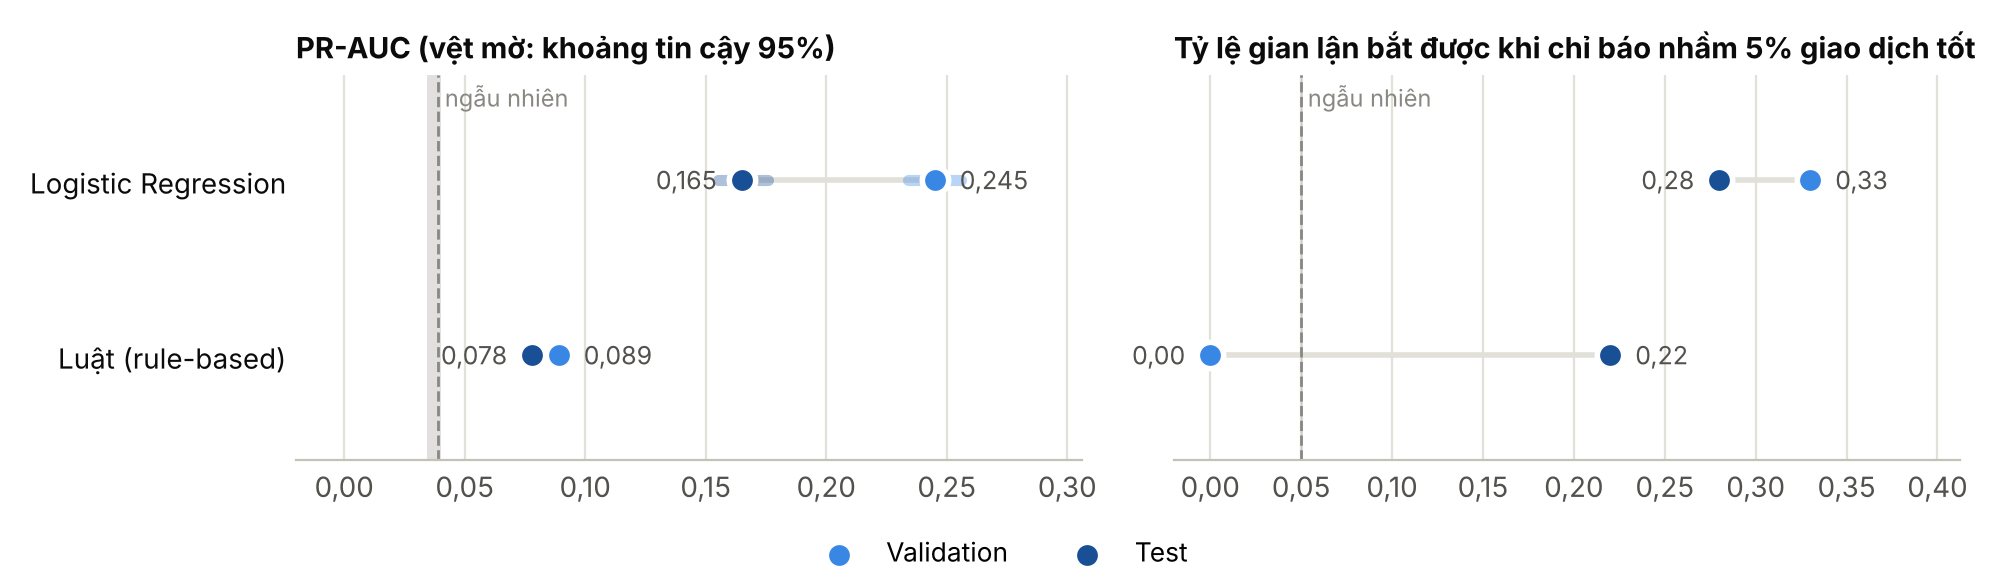
\includegraphics[width=0.95\linewidth]{figures/results.png}
\caption{Validation (nhạt) và test (đậm). Vùng xám: mức của bộ phân loại ngẫu nhiên.}\label{fig:fraud}
\end{figure}

Logistic Regression vượt baseline luật với khoảng tin cậy không chồng nhau, và trên test đạt khoảng 4,8 lần mức ngẫu nhiên. Kết quả giảm từ validation sang test, kể cả ở chỉ số không phụ thuộc tỷ lệ lớp (recall tại FPR 5\%: 0,33 xuống 0,28), cho thấy mức giảm không chỉ do tỷ lệ gian lận thấp hơn mà phù hợp với trôi khái niệm \cite{gama}. Giá trị 0 của baseline luật trên validation là do điểm luật chỉ nhận vài mức rời rạc: mức chặt nhất báo nhầm 5,1\% giao dịch hợp lệ, vượt ràng buộc 5\%. Có hai lần chạy test (\code{run-515a1190a0a4}, trước khi thêm chỉ số FPR, và \code{run-d6faa4699008}); mọi chỉ số chung trùng khớp, nên lần thứ hai không được dùng để chọn lại mô hình.

\paragraph{Gradient Boosting} Lần chạy \code{run-f8807cb6f780} chọn $\nu=0{,}1$, 400 cây, 15 lá (PR-AUC validation 0,497 [0,483; 0,514]); cấu hình được chốt trước khi mở tập test một lần. Trên test, PR-AUC đạt \textbf{0,408} [0,390; 0,424], gấp khoảng 2,5 lần Logistic Regression với khoảng tin cậy không giao nhau; recall tại FPR 5\% là 0,51 (Logistic Regression 0,28). Mức giảm từ validation sang test (0,089) tương đương của Logistic Regression (0,080). Lưới mở rộng đến 1.200 cây không cho kết quả tốt hơn. Trên validation, đặc trưng lịch sử thực thể tự dựng không cải thiện đo được: bỏ các cột đếm \code{C1}--\code{C14} làm PR-AUC rơi từ 0,497 xuống 0,158, cho thấy chúng đã chứa phần lớn thông tin theo thực thể; khoá có \code{D1n} cho +0,0114 khi lấy mẫu theo dòng nhưng [$-$0,0026; +0,0249] khi lấy mẫu theo cụm \code{card1}. Thống kê tổng hợp theo thực thể tính chỉ trên giao dịch trước đó (độ lệch chuẩn, z-score số tiền, số giá trị khác nhau) cũng không giúp (PR-AUC 0,497--0,498).

\paragraph{Thí nghiệm rò rỉ} Bảng~\ref{tab:leak} báo cáo lần chạy \code{leak-827d929eaa73}, chỉ trên validation.

\begin{table}[H]\centering
\caption{Thí nghiệm rò rỉ trên validation (118.108 dòng), Logistic Regression của baseline.}\label{tab:leak}
\begin{tabular}{@{}lcc@{}}
\toprule
Biến thể & PR-AUC [95\% CI] & Chênh \\ \midrule
Đúng quy tắc & 0,245 [0,235; 0,257] & +0,000 \\
(a) Chia ngẫu nhiên & 0,177 [0,168; 0,190] & $-$0,068 \\
(b) Tiền xử lý trên mọi dòng & 0,244 [0,234; 0,256] & $-$0,001 \\
(c) Mã hoá \code{card1} ngoài fold & 0,252 [0,242; 0,264] & +0,007 \\
(d) Mã hoá \code{card1} rò nhãn & 0,308 [0,297; 0,321] & \textbf{+0,063} \\
(e) Khoảng trống 7 / 14 ngày & 0,244 / 0,241 & $-$0,002 / $-$0,004 \\ \bottomrule
\end{tabular}
\end{table}

Rò nhãn qua mã hoá theo nhãn (d) là biến thể duy nhất làm điểm tăng rõ. Biến thể (b) và (e) đổi PR-AUC không quá 0,004, nhỏ hơn độ rộng khoảng tin cậy. Ngược kỳ vọng, chia ngẫu nhiên (a) cho điểm \emph{thấp hơn}. Chẩn đoán (chỉ train và validation) cho thấy hai validation là hai tập dòng khác nhau: đổi cách huấn luyện chỉ đổi PR-AUC 0,001--0,012, còn đổi tập đánh giá đổi khoảng 0,07; tỷ lệ gian lận giải thích khoảng 0,012, và các tuần đầu có tỷ lệ gian lận thấp (1,9--2,8\%) giải thích khoảng một nửa mức chênh (phân tích sau khi xem dữ liệu theo tuần); khoảng 0,03 còn lại chưa giải thích. Recall tại FPR 5\% gần như không đổi, nên không có bằng chứng mô hình kém đi. 98,7\% dòng validation có \code{card1} đã gặp trong train (85,9\% với \code{card1}+\code{addr1}+\code{P\_emaildomain}).

\subsection{Giám sát độ ổn định thanh toán}\label{sec:res-rel}
Ngưỡng chọn trên bộ tuning là 7 cho D-A và 8 cho D-B (gộp $k=2$ khung, tức 30 phút). Cấu hình được commit lúc 14:27:02 UTC, trước lần chạy duy nhất trên bộ report lúc 14:27:31 UTC.

\begin{table}[H]\centering
\caption{Phát hiện sự cố. Tuning: \code{det-3ddc26cff253}; report: \code{det-08335c6af086}.}\label{tab:det}
\begin{tabular}{@{}lcc@{}}
\toprule
Detector & Tuning (phát hiện; báo nhầm/ngày) & Report (phát hiện; báo nhầm/ngày) \\ \midrule
D-B gộp cửa sổ & 3/4; 0,00 & \textbf{2/4; 0,00} \\
D-A z-score bền vững & 2/4; 1,00 & 0/4; 2,00 \\ \bottomrule
\end{tabular}
\end{table}

\begin{table}[H]\centering
\caption{Từng sự cố trên bộ report (điểm cao nhất D-A / D-B; ngưỡng 7 / 8).}\label{tab:det-each}
\begin{tabular}{@{}llccc@{}}
\toprule
Sự cố & Đối tượng & Điểm & D-A & D-B \\ \midrule
Provider lỗi x3, 60 phút & \code{prov\_003} & 5,3 / 13,9 & trượt & phát hiện sau 15 phút \\
Độ trễ tăng x2,5, 2 giờ & \code{prov\_002} & 6,0 / 12,7 & trượt & phát hiện sau 30 phút \\
Mất lưu lượng QR x5, 2 giờ & QR & 3,6 / 6,6 & trượt & trượt \\
Provider lỗi x1,5, 2 giờ & \code{prov\_002} & 2,2 / 2,6 & trượt & trượt \\ \bottomrule
\end{tabular}
\end{table}

\begin{figure}[H]\centering
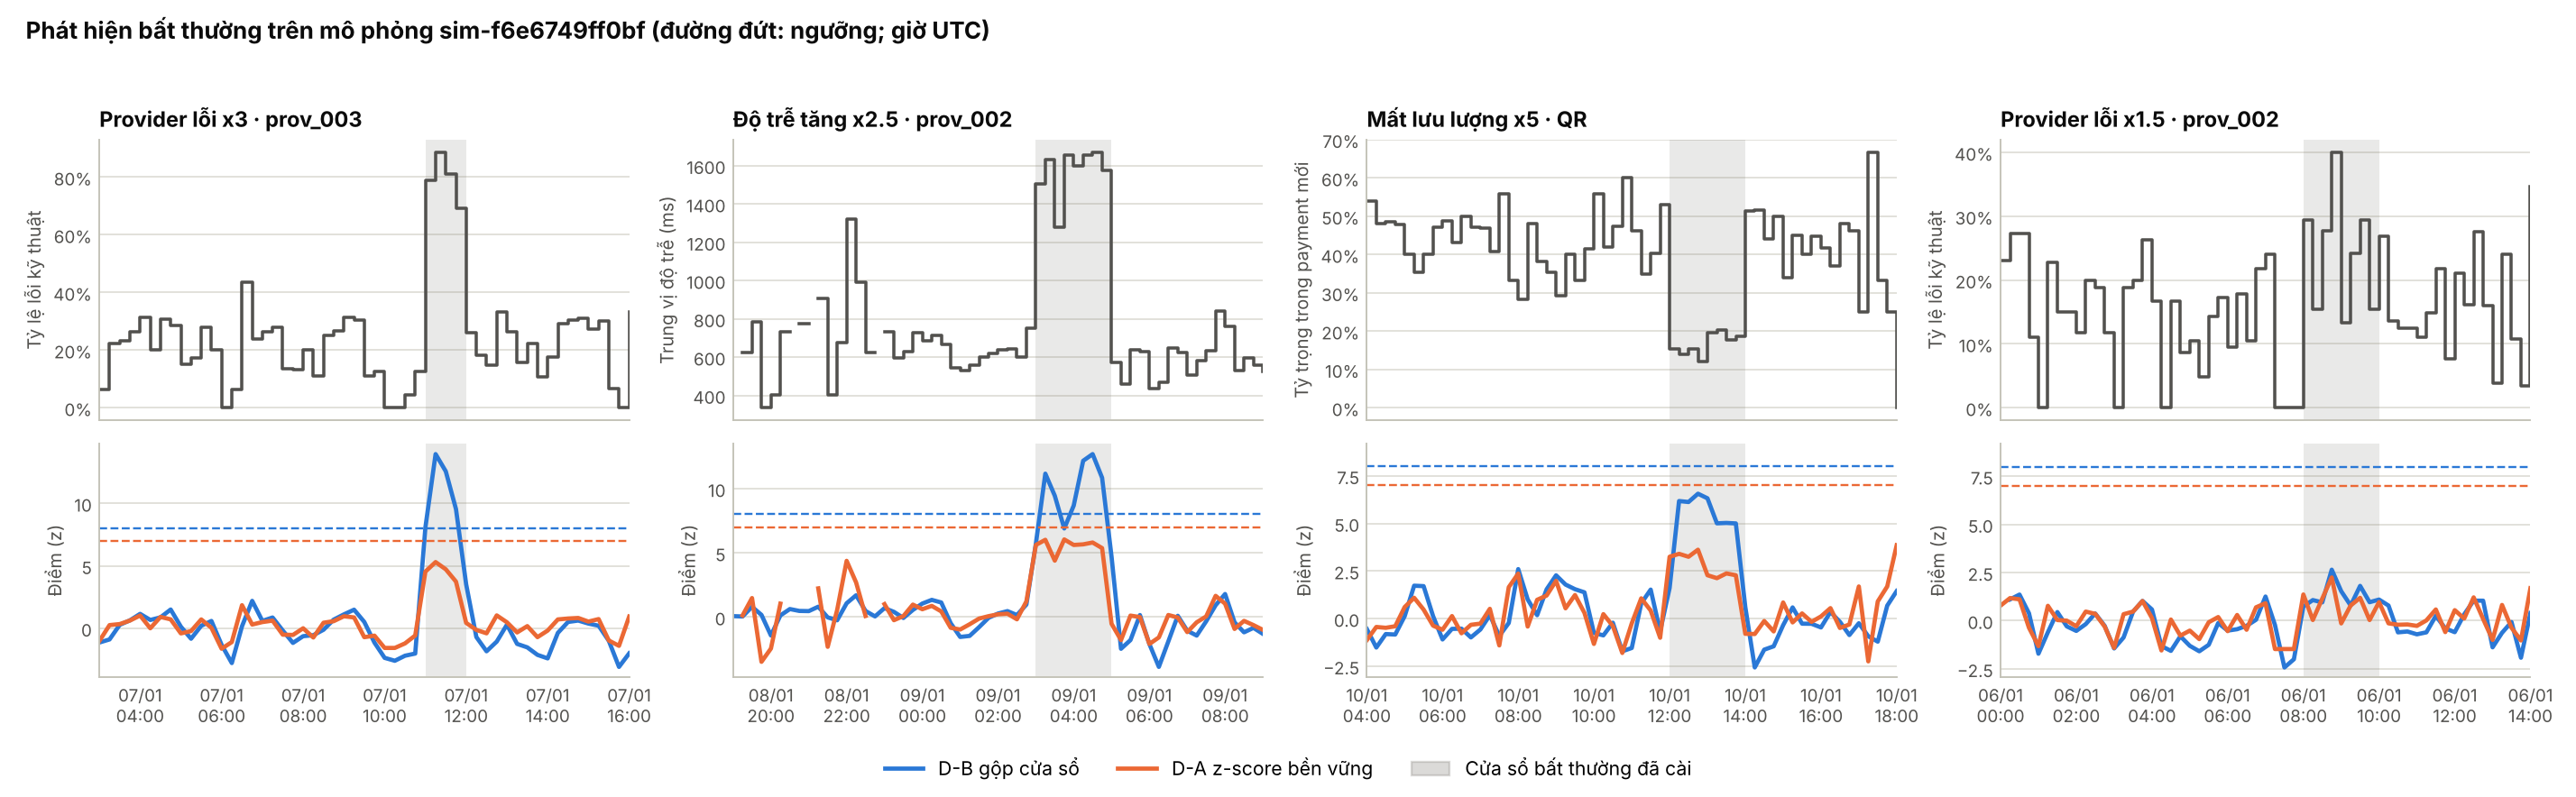
\includegraphics[width=\linewidth]{figures/stage-d-report.png}
\caption{Bộ report: KPI của đối tượng bị ảnh hưởng quanh mỗi sự cố (trên) và điểm của hai detector (dưới). Vùng xám là cửa sổ sự cố cài sẵn; đường đứt là ngưỡng.}\label{fig:det}
\end{figure}

D-B tốt hơn D-A trên cả hai bộ. Cả 14 báo động nhầm của D-A trên bộ report rơi vào 01:45--05:45 giờ Việt Nam, khi mỗi khung chỉ có vài attempt; ngoài các cửa sổ sự cố, điểm cao nhất của D-A là 9,4 so với 3,8 của D-B. Hai sự cố bị D-B bỏ sót có nguyên nhân khác nhau:
\begin{itemize}
  \item \emph{Mất lưu lượng.} Tỷ trọng QR giảm từ 44,0\% (24 giờ trước) xuống 16,6\%, nhưng mỗi cửa sổ 30 phút chỉ có khoảng 110 payment mới, nên điểm đạt 6,6 dưới ngưỡng 8. Ngưỡng được chọn trên bộ tuning, vốn không có loại sự cố này; chuỗi tỷ trọng có mức nhiễu thấp hơn (điểm cao nhất ngoài sự cố 3,3 trên bộ tuning), nên một ngưỡng chung tỏ ra quá khắt khe cho nó.
  \item \emph{Sự cố yếu.} Tỷ lệ lỗi kỹ thuật của \code{prov\_002} chỉ tăng từ 16,2\% lên 24,8\% (35/141 attempt); gộp cả 2 giờ, theo~\eqref{eq:binz}, được $z\approx 2{,}8$, thấp xa ngưỡng cần để không báo nhầm. Ở mức lưu lượng này, sự cố x1,5 nằm dưới giới hạn phát hiện.
\end{itemize}
Theo giao thức, ngưỡng không được chỉnh lại sau khi xem kết quả report.

% ===================================================================== 6
\section{Thảo luận}
\paragraph{Bài học} (1) Với dữ liệu thay đổi theo thời gian, kết quả validation lạc quan hơn kết quả test; giữ tập test cho một lần đo cuối là điều kiện để con số báo cáo có ý nghĩa. (2) Trong phát hiện bất thường trên tỷ lệ, việc mô hình hoá lượng dữ liệu phía sau mỗi tỷ lệ (D-B) mang lại nhiều hơn việc chọn ngưỡng khéo cho một thống kê không biết đến cỡ mẫu (D-A). (3) Một bộ đánh giá độc lập có loại sự cố chưa gặp lộ ra điểm mù mà bộ chỉnh ngưỡng không cho thấy.

\paragraph{Các mối đe doạ đến tính hợp lệ}
\begin{itemize}
  \item \emph{Dữ liệu giả lập}: mọi tham số do người làm đặt; kết quả là kiểm chứng trên bất thường đã biết, không phải hiệu năng thực tế.
  \item \emph{Cỡ mẫu sự cố}: 4 + 4 sự cố; các tỷ lệ phát hiện chỉ có tính minh hoạ.
  \item \emph{Giả định độc lập}: D-B coi các attempt độc lập, trong khi retry của cùng payment có tương quan; điểm $z$ có thể bị phóng đại nhẹ.
  \item \emph{Nhãn IEEE-CIS}: theo mô tả của ban tổ chức, nhãn lan sang các giao dịch sau của cùng tài khoản, và cùng một thẻ có thể xuất hiện ở nhiều tập; chia theo thời gian không loại bỏ hiện tượng này. Thí nghiệm ở Mục~\ref{sec:leak} được thiết kế để đo nó.
  \item \emph{Tái lập}: dữ liệu giả lập giống hệt từng byte chỉ khi cùng phiên bản numpy; định danh lần chạy không chứa phiên bản thư viện, và thí nghiệm rò rỉ chạy lại trên môi trường khác lệch $\pm$0,001 ở 3 biến thể.
\end{itemize}

% ===================================================================== 7
\section{Hướng phát triển}
\begin{enumerate}
  \item Kiểm chứng phần còn lại của mức chênh khi chia ngẫu nhiên, và kiểm tra khoá có \code{D1n} trên giai đoạn dữ liệu mới với cấu hình và tập test mới.
  \item Ngưỡng riêng cho từng loại KPI, đánh giá trên một bộ report mới.
  \item Detector có mùa vụ \cite{fpp} hoặc tích luỹ (CUSUM) cho sự cố yếu nhưng kéo dài.
  \item API chấm điểm chỉ hỗ trợ quyết định, không tự động chặn giao dịch.
  \item Đặc trưng theo thẻ chỉ dùng thông tin quá khứ; LightGBM; hiệu chỉnh xác suất.
  \item dbt khi số mô hình dữ liệu tăng; luồng sự kiện thời gian thực; theo dõi trôi dữ liệu; dữ liệu thật khi được phê duyệt.
\end{enumerate}

% ===================================================================== 8
\section{Kết luận}
Bài báo trình bày một nền tảng dữ liệu tái lập được cho hai bài toán thanh toán và một giao thức đánh giá chung. Trên IEEE-CIS, Logistic Regression đạt PR-AUC 0,165 trên tập kiểm tra, hơn gấp đôi baseline luật (0,078), và Gradient Boosting cùng đặc trưng đạt 0,408. Trên dữ liệu giả lập, điểm số nhị thức gộp cửa sổ phát hiện các sự cố về lỗi và độ trễ trong 15--30 phút mà không báo nhầm, vượt rõ z-score bền vững; đồng thời, giao thức chỉnh ngưỡng và báo cáo trên hai bộ dữ liệu tách biệt cho thấy rõ giới hạn của nó với sự cố mất lưu lượng và sự cố yếu.

\section*{Lời cảm ơn}
Tác giả cảm ơn người hướng dẫn và đơn vị thực tập. Mã nguồn được phát triển với sự hỗ trợ của một công cụ lập trình có trí tuệ nhân tạo; mọi quyết định thiết kế, cấu hình được chốt và số liệu báo cáo do tác giả duyệt.

% ===================================================================== Tài liệu
\begin{thebibliography}{99}\small
\bibitem{saito} T. Saito, M. Rehmsmeier. The precision-recall plot is more informative than the ROC plot when evaluating binary classifiers on imbalanced datasets. \emph{PLOS ONE}, 10(3), 2015.
\bibitem{jesus} S. Jesus et al. Turning the tables: Biased, imbalanced, dynamic tabular datasets for ML evaluation. \emph{NeurIPS Datasets and Benchmarks}, 2022.
\bibitem{kaufman} S. Kaufman, S. Rosset, C. Perlich, O. Stitelman. Leakage in data mining: Formulation, detection, and avoidance. \emph{ACM TKDD}, 6(4), 2012.
\bibitem{kapoor} S. Kapoor, A. Narayanan. Leakage and the reproducibility crisis in machine-learning-based science. \emph{Patterns}, 4(9), 2023.
\bibitem{gama} J. Gama, I. Žliobaitė, A. Bifet, M. Pechenizkiy, A. Bouchachia. A survey on concept drift adaptation. \emph{ACM Computing Surveys}, 46(4), 2014.
\bibitem{grinsztajn} L. Grinsztajn, E. Oyallon, G. Varoquaux. Why do tree-based models still outperform deep learning on typical tabular data? \emph{NeurIPS Datasets and Benchmarks}, 2022.
\bibitem{handbook} Y.-A. Le Borgne, W. Siblini, B. Lebichot, G. Bontempi. \emph{Reproducible Machine Learning for Credit Card Fraud Detection: Practical Handbook}. Université Libre de Bruxelles, 2022.
\bibitem{dalpozzolo} A. Dal Pozzolo, G. Boracchi, O. Caelen, C. Alippi, G. Bontempi. Credit card fraud detection: A realistic modeling and a novel learning strategy. \emph{IEEE TNNLS}, 29(8), 2018.
\bibitem{chandola} V. Chandola, A. Banerjee, V. Kumar. Anomaly detection: A survey. \emph{ACM Computing Surveys}, 41(3), 2009.
\bibitem{lavin} A. Lavin, S. Ahmad. Evaluating real-time anomaly detection algorithms: The Numenta Anomaly Benchmark. \emph{ICMLA}, 2015.
\bibitem{wu} R. Wu, E. Keogh. Current time series anomaly detection benchmarks are flawed and are creating the illusion of progress. \emph{IEEE TKDE}, 2021.
\bibitem{sre} B. Beyer, C. Jones, J. Petoff, N. R. Murphy (eds.). \emph{Site Reliability Engineering}. O'Reilly, 2016.
\bibitem{fpp} R. J. Hyndman, G. Athanasopoulos. \emph{Forecasting: Principles and Practice}, 3rd ed. OTexts, 2021.
\bibitem{paysim} E. Lopez-Rojas, A. Elmir, S. Axelsson. PaySim: A financial mobile money simulator for fraud detection. \emph{EMSS}, 2016.
\bibitem{jsonschema} JSON Schema Specification, Draft 2020-12. \url{https://json-schema.org/specification}.
\bibitem{kleppmann} M. Kleppmann. \emph{Designing Data-Intensive Applications}. O'Reilly, 2017.
\bibitem{ieee} IEEE Computational Intelligence Society, Vesta. IEEE-CIS Fraud Detection (Kaggle), 2019. \url{https://www.kaggle.com/c/ieee-fraud-detection}.
\end{thebibliography}

\appendix
\section{Tái lập}
Mã nguồn và cấu hình nằm trong kho mã nêu ở đầu bài. Các bước: \code{make setup}; \code{make baseline} và \code{make baseline-final} (Product 02); \code{make simulate}, \code{make ingest}, \code{make kpi}, \code{make tune}, \code{make detect}, \code{make detect-report} (Product 01); \code{make leakage}, \code{make gbm} (thí nghiệm rò rỉ, Gradient Boosting); \code{make dashboard}. Kiểm thử: 372 test chạy trên Python 3.11 và 3.13.

\end{document}
